\documentclass[border=8pt]{standalone}
\usepackage{tikz}
\usetikzlibrary{arrows.meta,positioning,fit,calc,backgrounds}
\usepackage{lmodern}
\usepackage{xcolor}
\usepackage{siunitx}
\definecolor{navy}{HTML}{17365D}
\definecolor{teal}{HTML}{0F6B6D}
\definecolor{amber}{HTML}{B56B00}
\definecolor{crimson}{HTML}{A51C30}
\definecolor{softgray}{HTML}{F3F5F7}
\definecolor{lightblue}{HTML}{E8F0FE}
\definecolor{lightgreen}{HTML}{E8F5E9}
\definecolor{lightorange}{HTML}{FFF3E0}
\definecolor{lightred}{HTML}{FFEBEE}
\begin{document}
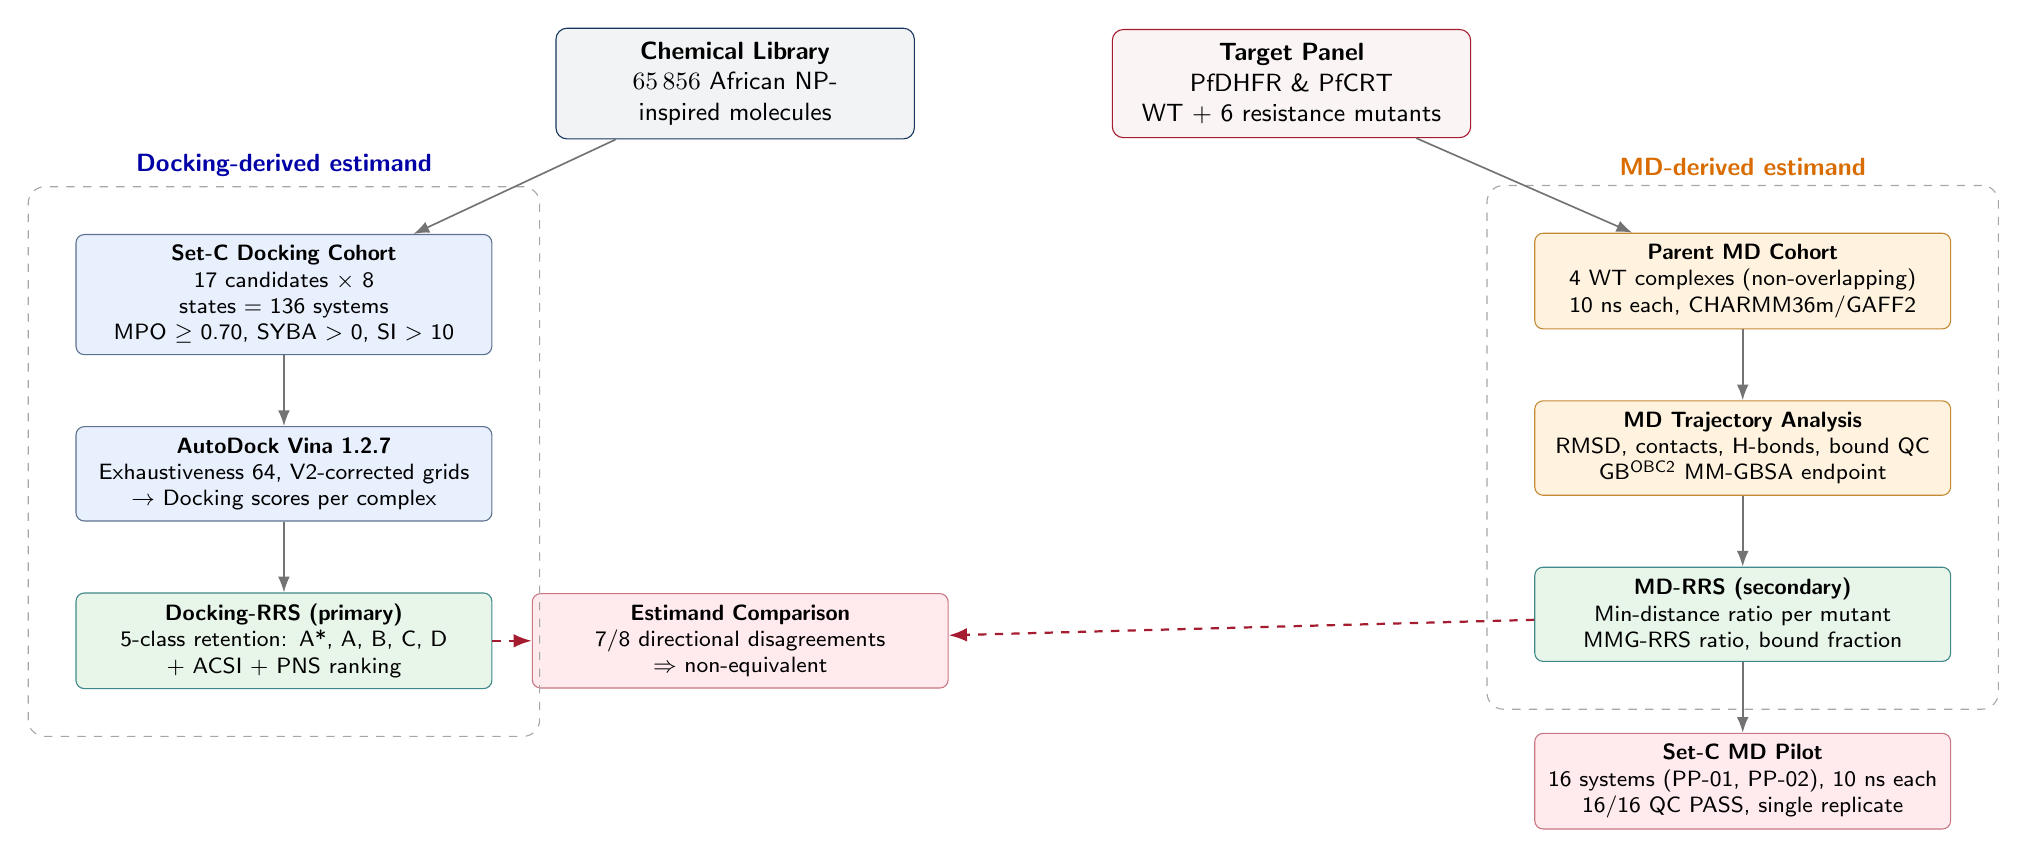
\begin{tikzpicture}[
  font=\sffamily,
  >=Latex,
  node distance=9mm and 12mm,
  every node/.style={line width=0.4pt},
  % Styles
  source/.style={draw=navy, rounded corners=4pt, fill=navy!6, align=center,
    text width=42mm, minimum height=11mm, inner sep=5pt, font=\small\sffamily},
  source2/.style={draw=crimson, rounded corners=4pt, fill=crimson!5, align=center,
    text width=42mm, minimum height=11mm, inner sep=5pt, font=\small\sffamily},
  method/.style={draw=navy!70, rounded corners=3pt, fill=lightblue, align=center,
    text width=50mm, minimum height=10mm, inner sep=4pt, font=\footnotesize\sffamily},
  mdbox/.style={draw=amber!80, rounded corners=3pt, fill=lightorange, align=center,
    text width=50mm, minimum height=10mm, inner sep=4pt, font=\footnotesize\sffamily},
  result/.style={draw=teal!80, rounded corners=3pt, fill=lightgreen, align=center,
    text width=50mm, minimum height=10mm, inner sep=4pt, font=\footnotesize\sffamily},
  secondary/.style={draw=crimson!60, rounded corners=3pt, fill=lightred, align=center,
    text width=50mm, minimum height=10mm, inner sep=4pt, font=\footnotesize\sffamily},
  boundary/.style={draw=black!35, dashed, rounded corners=6pt, inner sep=6mm},
  arrow/.style={->, semithick, draw=black!55},
  arrowdash/.style={->, semithick, draw=black!55, dashed},
  % Label styles
  blabel/.style={font=\scriptsize\sffamily\color{blue!65!black}, midway, left, xshift=-2pt},
  olabel/.style={font=\scriptsize\sffamily\color{orange!85!black}, midway, right, xshift=2pt},
]

% === ROW 1: Inputs ===
\node[source] (library) {
  \textbf{Chemical Library}\\
  \num{65856} African NP-inspired molecules
};
\node[source2, right=25mm of library] (targets) {
  \textbf{Target Panel}\\
  PfDHFR \& PfCRT\\
  WT + 6 resistance mutants
};

% === ROW 2: Cohorts ===
\node[method, below left=12mm and 8mm of library] (setc) {
  \textbf{Set-C Docking Cohort}\\
  17 candidates $\times$ 8 states = 136 systems\\
  MPO $\geq$ 0.70, SYBA $>$ 0, SI $>$ 10
};
\node[mdbox, below right=12mm and 8mm of targets] (parent) {
  \textbf{Parent MD Cohort}\\
  4 WT complexes (non-overlapping)\\
  10 ns each, CHARMM36m/GAFF2
};

% === ROW 3: Methods ===
\node[method, below=9mm of setc] (docking) {
  \textbf{AutoDock Vina 1.2.7}\\
  Exhaustiveness 64, V2-corrected grids\\
  $\rightarrow$ Docking scores per complex
};
\node[mdbox, below=9mm of parent] (traj) {
  \textbf{MD Trajectory Analysis}\\
  RMSD, contacts, H-bonds, bound QC\\
  GB$^{\text{OBC2}}$ MM-GBSA endpoint
};

% === ROW 4: Outputs ===
\node[result, below=9mm of docking] (rrs) {
  \textbf{Docking-RRS (primary)}\\
  5-class retention: A*, A, B, C, D\\
  + ACSI + PNS ranking
};
\node[result, below=9mm of traj] (mdresult) {
  \textbf{MD-RRS (secondary)}\\
  Min-distance ratio per mutant\\
  MMG-RRS ratio, bound fraction
};

% === ROW 5: Pilot ===
\node[secondary, below=9mm of mdresult] (pilot) {
  \textbf{Set-C MD Pilot}\\
  16 systems (PP-01, PP-02), 10 ns each\\
  16/16 QC PASS, single replicate
};

% === Dashed lines for non-equivalence ===
\node[secondary, right=5mm of rrs] (comp) {
  \textbf{Estimand Comparison}\\
  7/8 directional disagreements\\
  $\Rightarrow$ non-equivalent
};

% === Boundaries ===
\node[boundary, fit=(setc) (docking) (rrs),
  label={[blue!65!black]above:\small\sffamily\textbf{Docking-derived estimand}}] (dockbox) {};
\node[boundary, fit=(parent) (traj) (mdresult),
  label={[orange!85!black]above:\small\sffamily\textbf{MD-derived estimand}}] (mdbox) {};

% === Arrows ===
\draw[arrow] (library) -- (setc);
\draw[arrow] (targets) -- (parent);
\draw[arrow] (setc) -- (docking);
\draw[arrow] (docking) -- (rrs);
\draw[arrow] (parent) -- (traj);
\draw[arrow] (traj) -- (mdresult);
\draw[arrow] (mdresult) -- (pilot);
\draw[arrowdash, thick, crimson] (rrs) -- (comp);
\draw[arrowdash, thick, crimson] (mdresult) -- (comp);

% === Vertical annotation ===
\node[font=\scriptsize\sffamily, rotate=90, above=2mm of dockbox] at ($(dockbox.north west)!0.5!(dockbox.north east)$) {};
\node[font=\scriptsize\sffamily, rotate=90, above=2mm of mdbox] at ($(mdbox.north west)!0.5!(mdbox.north east)$) {};

\end{tikzpicture}
\end{document}
